\documentclass[12pt,journal]{IEEEtran}
\usepackage[utf8]{inputenc}
\usepackage[cmex10]{amsmath}
\usepackage{xcolor, graphicx, hyperref}
\hyphenation{op-tical net-works semi-conduc-tor}
\begin{document}

\title{Predicting a Song's Popularity by Using Logistic Regression and Random Forest Models on Spotify Performance Charts}
\author{
\textcolor{white}{.} Carlos Flores, \hspace{5mm} Johannes Limano, \hspace{7mm}
 Martin Lopez, \hspace{17mm} Daniel Rivas \hspace{6mm} \textcolor{white}{.} \\
cflores28@uh.edu \hspace{2mm} jdlimano@uh.edu \hspace{2mm} 
mjimenez9@uh.edu \hspace{2mm} derivassanchez@uh.edu
}

\markboth{Group Project Report, November 29, 2020}
{}

\IEEEtitleabstractindextext{%
\begin{abstract}
The American Music industry is known for being fickle and constantly changing. Historians have noted that trends have emerged in popular music over time. These fads come into prominence for years and then become replaced by another trend. Detecting emerging patterns in the songs that become popular has many important applications, particularly in artist development. In order to determine a song's success, two methods were used to predict the track's popularity, Random Under Sampling and  SMOTEENN Techniques. The data was used to build Logistic Regression models and able to yield good results, with 78\% to 82\% accuracy in classifying top tracks and unpopular tracks.
\end{abstract}

% Note that keywords are not normally used for peer review papers.
\begin{IEEEkeywords}
Feature Selection, Dimensionality Reduction, Data Preprocessing, FuzzyWuzzy String Comparison, SMOTE Oversampling, SMOTEEN Undersampling, Bootstrapping, Logistic Regression.
\end{IEEEkeywords}}

% make the title area
\maketitle
\IEEEdisplaynontitleabstractindextext

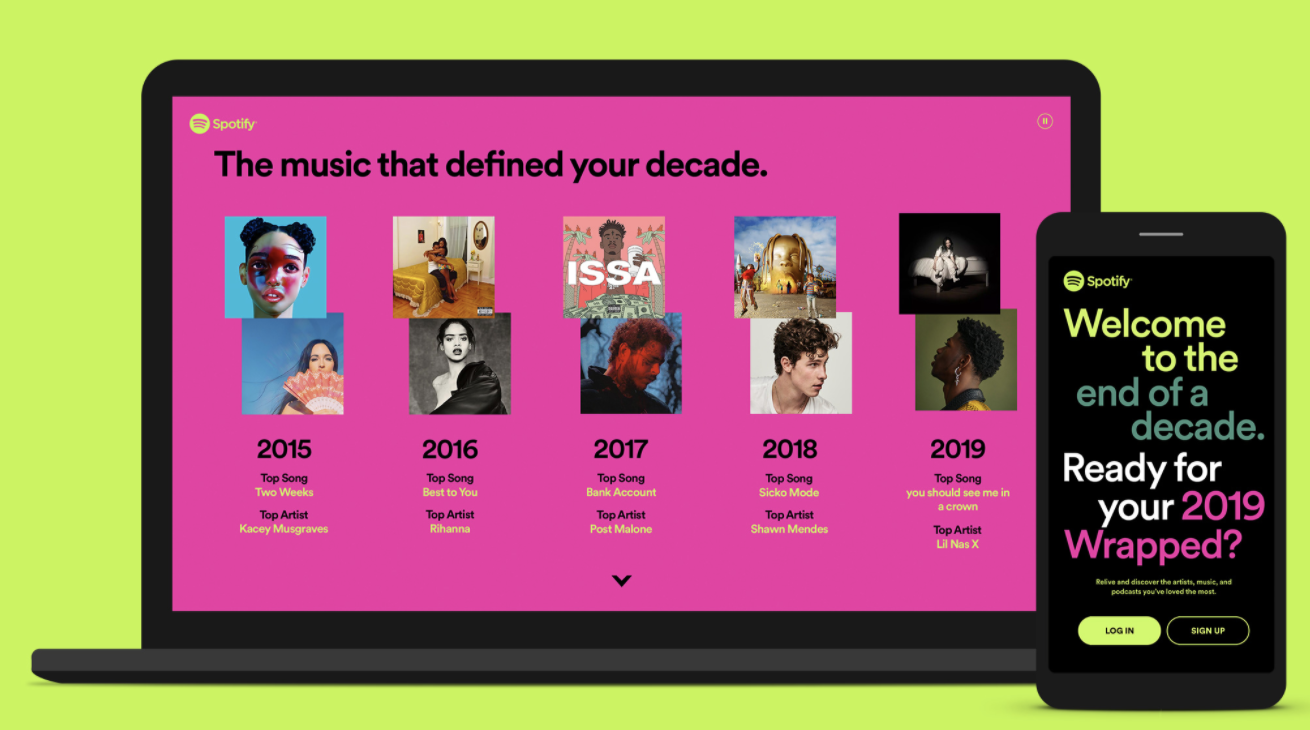
\includegraphics[width=.9\linewidth, height=.6\linewidth]{ss1}

\section{Introduction}
\IEEEPARstart{S}{potify} publishes their top tracks of the year in December. This acts as an annual summary to gauge user activity on the platform. The Spotify report is considered to be highly influential for the music industry as a whole - given that consumer behaviors have changed from radio plays towards online track streaming. We have culled the top Spotify tracks into a single dataset onto which we will build our predictive models.

\section{Preprocessing}
\IEEEPARstart{H}{owever}, the data only includes the tracks that have performed well amongst Spotify listeners. Our model would surely need to incorporate unpopular tracks to understand song popularity on a holistic level than a singular perspective. By combining the dataset with other sources to include unpopular tracks we are able to train the models to identify 'good' and 'bad' songs. We used various preprocessing techniques to merge the dataset in an appropriate manner. That of which include:


\subsection{Feature Creation}
We have created a new binary feature called 'toptracks' as our class label. A toptracks of 'Y' indicates that the song was popular on Spotify, while a toptracks value of 'N' indicates that the song was not popular enough to be on the top tracks of the year.

\subsection{Normalizing Features}
After merging the datasets we normalized the names and standardized the units of measurement for each column. Doing so is critical to the integrity of the project as the different data sources had slight differences in verbiage for the equivalent feature. To achieve this we used the FuzzyWuzzy package which contains a number of tools to compare strings and compute the standard Levenshtein distance similarity ratio between them. There are even other useful tools that allow us to compare substrings that are in different arrangements. 

Another viable python package that was considered was Difflib which contains a very similar toolset to compare strings and substrings. However, we ultimately chose the former as it is far more popular, not to mention that the Levenshtein algorithm has a better performing complexity than difflib.SequenceMatcher for words that contain out-of-order characters.

\subsection{Merging Datasets}
We decided to add another feature (column) in our unlabeled main dataset by merging a collection of top charts datasets from top tracks of 2010 to 2019. Before we merged a collection of top charts datasets from top tracks of 2010 to 2019, we normalized our column names using fuzzy-wuzzy library (see \S2b \textit{Normalizing Features}). This column normalization is important since among top charts datasets from top tracks of 2010 to 2019, they have different lists of column names. Then the merged top chart dataset acts as a lookup table for the unlabeled main dataset.

We then compare the artist, title and year of the track of each track in our unlabeled main dataset with the merged top chart dataset by using fuzzy-wuzzy library again. If the track from the unlabeled main dataset exists in the merged top chart dataset, we then mark this track’s new feature topcharts as a Y (yes) for being in the top chart. Otherwise, this feature will be marked as a N (no) which indicates that this track is not in the top chart. \\

As a result, we have obtained our main labeled dataset.

\subsection{Feature Elimination}
Some of the features were used by Spotify but not useful in our model. Those attributes were dropped to reduce the size of the data set:\\
\begin{enumerate}
	\item id - This is a unique identifier used by Spotify's in-house metrics and irrelevant for our use.
	\item release\_date - Redundant feature; we have another feature, 'Year,' that works better with numerical data.
	\item title - Nominal Variable with no viable encoding function to create a dummy variable. The classification models would have trouble with nominal values and we dropped them from the data set for that reason.
	\item artist - Same reason as described for 'title.'
\end{enumerate}

\section{Data Exploration}
\IEEEPARstart{A}{} pairplot and histogram evaluation provided some trends in the dataset:\\

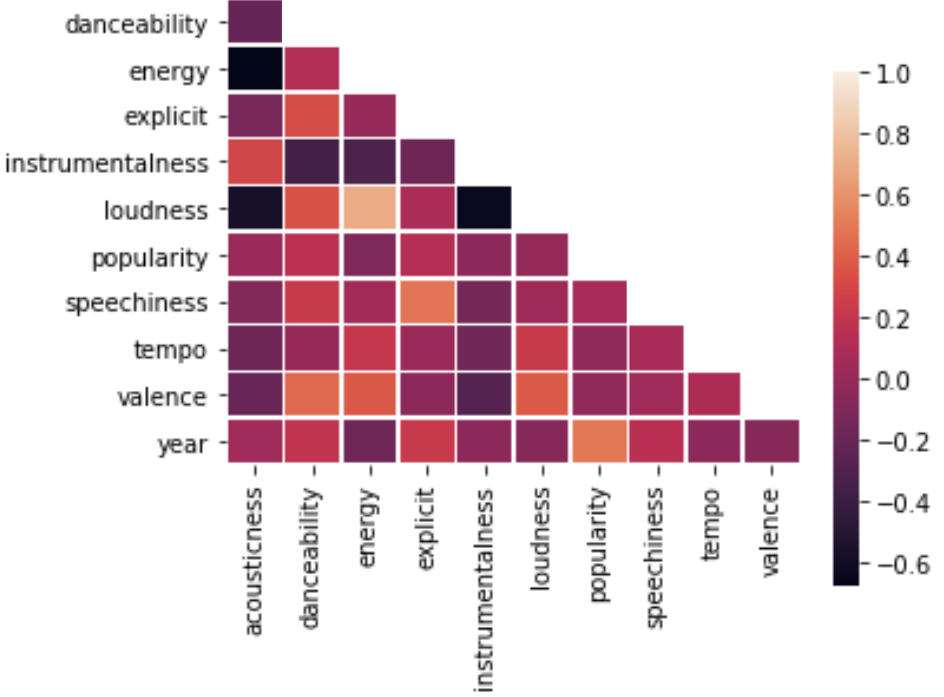
\includegraphics[width=\linewidth]{ss2}
\begin{center}
	\textit{Figure 3a: Correlation Matrix \\for the Cleaned Dataset}
\end{center}

\subsection{Dimensionality Reduction}
The following quantitative features provided no correlation whatsoever and were dropped to reduce the complexity of the feature space:
\begin{enumerate}
	\item duration\_ms - The length of the track in milliseconds.
	\item key - The overall key in which the song is in.
	\item liveness - Detects the presence of an audience in the recording.
	\item mode - Indicates the modality(major or minor  melodic scale used in the track).\\
\end{enumerate}

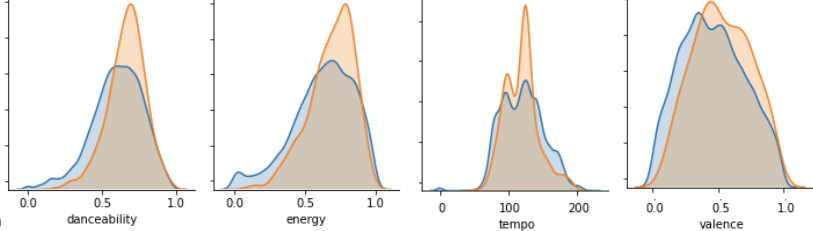
\includegraphics[width=\linewidth]{ss3}
\begin{center}
	\textit{Figure 3b: Supervised Histograms}
\end{center}

\subsection{Descriptive Statistics}
\begin{itemize}
	\item The cleaned dataset has a significant amount of colinearity between the following features: acousticness, danceability, energy, instrumentalness, loudness, tempo, valence.
	\item $96\%$ of all our class labels are '$No$' and leads to an overrepresentation in our model. We will address this problem in the next report.
	\item The histograms for tempo has a bimodal distribution for the toptracks. It seems that popular songs gravitate towards the same BPM ranges. Additionally, the danceability, energy, and valence histograms show positive kurtosis and a left skew. Overall, it could be said that popular songs are generally more danceable, have a higher energy, and a positive emotional tone.
	
\end{itemize}

\section{Feature Summary}
\IEEEPARstart{T}{he} following features were used in our models (the descriptions are taken directly from {\color{blue}\href{https://developer.spotify.com/documentation/web-api/reference/tracks/get-audio-features}{\underline{Spotify's official documentation}}} [1].\\

\begin{enumerate}
	\item acousticness - It is a confidence measure from 0.0 to 1.0  and represents the confidence in whether the track is acoustic or not (respectively).
	\item danceability - A value of 0.0 is least danceable and 1.0 is most danceable.
	\item energy - It is a measure from 0.0 to 1.0 and represents a perceptual measure of intensity and activity. Typically, energetic tracks feel fast, loud, and noisy.
	\item explicit - A binary value of 1 or 0 to represent if the song contains profanity or not.
	\item instrumentalness - The closer the instrumentalness value is to 1.0, the greater likelihood the track contains no vocal content. Values above 0.5 are intended to represent instrumental tracks, but confidence is higher as the value approaches 1.0.
	\item loudness - The overall loudness of the track rated in decibels. Values typically range between -60 and 0 db.
	\item popularity - A measure from 0.0 to 100.0 based on the number of times the track has been streamed.
	\item speechiness - A measure from 0.0 to 1.0. The more exclusively speech-like the recording (e.g. talk show, audio book, poetry), the closer to 1.0 the attribute value. Values above 0.66 describe tracks that are probably made entirely of spoken words. Values between 0.33 and 0.66 describe tracks that may contain both music and speech, either in sections or layered, including such cases as rap music. Values below 0.33 most likely represent music and other non-speech-like tracks.
	\item tempo - A measure of Beats per Minute (BPM) from 0.0 to 220.0.
	\item valence - A measure from 0.0 to 1.0 describing the musical positiveness conveyed by a track. Tracks with high valence sound more positive (e.g. happy, cheerful, euphoric), while tracks with low valence sound more negative (e.g. sad, depressed, angry).
	\item year - The year when the track was published, which is ranging from 2010 to 2020.

\end{enumerate}

\section{Resampling Techniques}
\IEEEPARstart{W}{e} did a lot with our data, we transformed, normalized, merged, and consolidated many different datasets into a single file. However, the class labels are not represented equally. The imbalance is so severe that the model is affected in many ways.


\begin{center}
	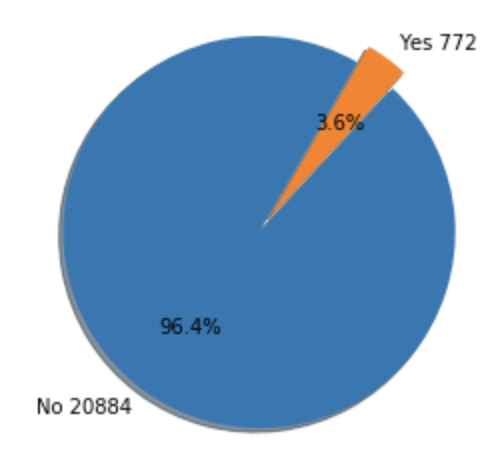
\includegraphics[width=.8\linewidth]{p1}
	
	\textit{Figure 5a: Proportion of TopTracks and non-TopTracks in the dataset}
\end{center}

\subsection{Imbalanced Datasets}
The dataset at this point is pretty unbalanced, we have around ~800 tracks that were in the topcharts (Y label, minority class) vs. ~22000 tracks that were not in the topcharts (N label, majority class). 

We did some modeling based on this dataset and the results we got weren’t very accurate for true positives due to the overwhelming non-topcharts tracks, which made our models biased to classifying everything as a non-topchart track.

To deal with such cases we need to balance our dataset  and make the minority class and majority class have approximately the same number of samples, such that our model is not biased towards any of them.


\subsection{Oversampling and Under-Sampling}
\begin{center}
	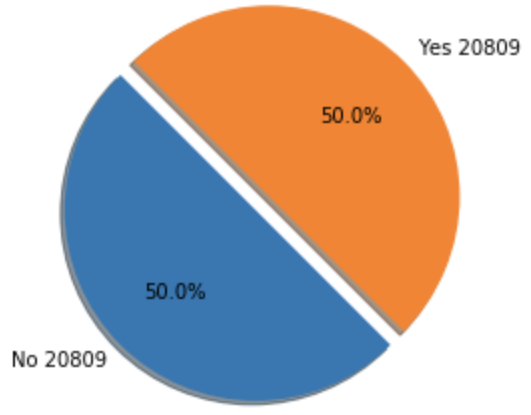
\includegraphics[width=.8\linewidth]{p3}
	
	\textit{Figure 5b.1: An Oversampled Example of Our Dataset by SMOTE}
\end{center}
Oversampling methods duplicate or create new synthetic examples in the minority class, whereas undersampling methods delete or merge examples in the majority class. Both types of resampling can be effective when used in isolation, although can be more effective when both types of methods are used together.

\begin{center}
	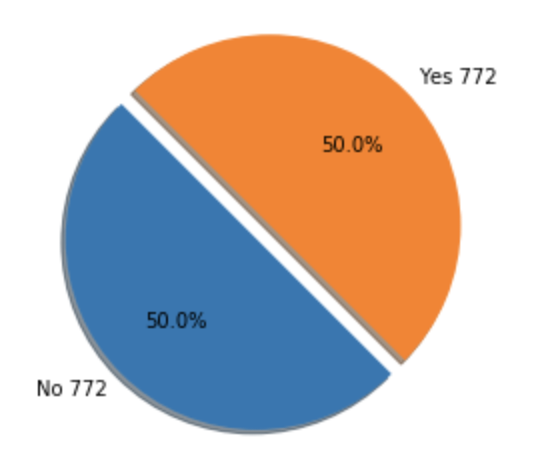
\includegraphics[width=.8\linewidth]{p2}
	
	\textit{Figure 5b.2: An Undersampled Example of Our Dataset by RUS Techniques}
\end{center}
Deciding between oversampling and under-sampling depends on the size of the data. For instance, we usually over-sample when the amount of samples in the minority class is not big enough; while we under-sample when the majority is too large[2].

\subsection{SMOTE and SMOTEENN}
Synthetic Minority Oversampling Technique (SMOTE) is one of the most popular oversampling methods. It takes samples from the minority class and uses k-nearest neighbors as well as interpolation to generate new points.

SMOTE combined with Edited Nearest Neighbors (SMOTEENN) can be used for under-sampling. It consists in using ENN for removing samples from the majority class that are misclassified by all its three (ENN k = 3) nearest neighbors.


\section{Model Training}
\IEEEPARstart{A}{fter} the dataset is balanced we should be ready to start training. Since some samples of our dataset are now synthetic, we have to be careful during modeling to prevent overfitting.

\begin{center}
	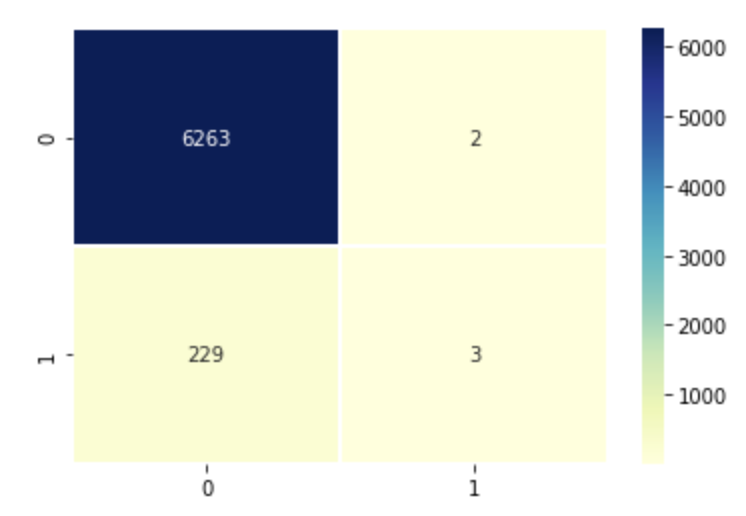
\includegraphics[width=.8\linewidth]{cm1}
	
	\textit{Figure 6a: The Confusion Matrix for the Initial Logistic Regression Model Shows a High Amount of False Negatives (229 / 232).}
\end{center}

\subsection{Initial Problems}
As mentioned previously, our first logistic regression model yields a 96.44\% accuracy score, and the model had a high amount of false-negatives. The initial model performed well in recognizing unpopular songs given the overwhelming majority in the dataset. So much so, that it was not able to identify popular songs at all. All of the class labels were predicted to be a non-TopTrack.

 It was precisely this result that made us aware of our imbalancing issues. The dataset that we use at this point is pretty unbalanced (in terms of the proportion between class label Y and N). We have 772 tracks that were in the top charts (Y label, minority class) vs. 20884 tracks that were not in the top charts (N label, majority class). The result we got was not very accurate for true positives due to the overwhelming amount of  non-top chart tracks, which made our logistic regression model biased toward classifying new data as a non-top chart track. To deal with such cases, we need to balance our dataset and make the minority class and majority class have approximately the same number of samples, such that our model is not biased towards any of the extreme points.

\subsection{Resampling Improvements}
\begin{center}
	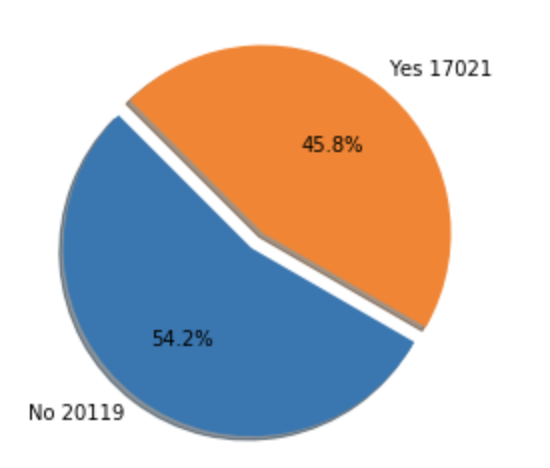
\includegraphics[width=.8\linewidth]{p4}
	
	\textit{Figure 6b.1: A Resampled Example of Our Dataset by SMOTEENN}
\end{center}
As pointed out in our previous logistic regression model, there is a severe imbalance to our dataset which leads to undesired results. We approach this issue by applying resampling techniques which will allow us to ensure the consistency of our model performance and statistics. As there are several resampling methods, one should always try several approaches and decide which technique is best for the problem at hand. Doing so will ensure that we have the best possible model for maximum predictive performance.

\begin{center}
	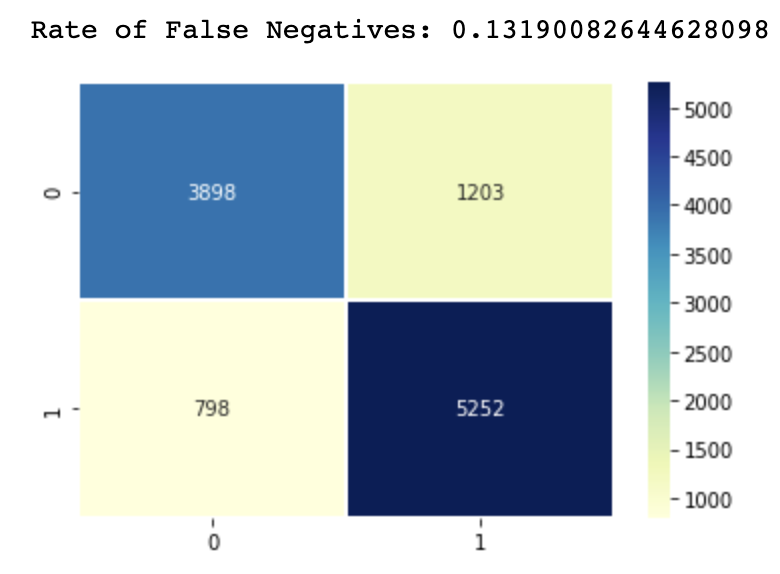
\includegraphics[width=.8\linewidth]{cm2}
	
	\textit{Figure 6b.2: The SMOTEENN Model Demonstrates a Much Lower Rate of False Positives (798 / 6050)}
\end{center}

To strike the best balance in our dataset we use SMOTEENN techniques to our dataset to train the models. This two-pronged approach will effectively minimize the amount of data that is lost from undersampling and lowers the amount of interpolation in oversampling known observations.

\section{Conclusion}
\IEEEPARstart{T}{he} resampled models demonstrated a higher rate of misclassification but the false negatives were significantly reduced. The raw data model simply predicted every observation to have a class label of the majority class. 

\begin{center}	
\begin{tabular} { | p {3 cm} | p {3 cm} | | p {3 cm} | }
\hline
\multicolumn{3} { | c |}{ML Model Performance Metrics}\\
\hline
Technique & \%Accuracy & \%False Negative \\
\hline
Raw Data & 96.44\% & 98.71\%  \\
RUS & 77.58\% & 21.55\% \\
SMOTE & 78.10\% & 18.91\% \\
SMOTEENN & 82.06\% & 13.19\% \\
\hline 
\end{tabular}
\textcolor{white}{.} \\

	\textit{Table 7a}
\end{center}

Meanwhile, the resampled models were able to build a meaningful regression scheme that identified popular songs with much more success. This improvement, at the cost of a higher rate of misclassification, is much more practical in a real-world scenario. It would be more important to avoid Type II errors and have a ML model that can correctly identify popular songs. The SMOTEEN Linear Regression model would work much better for professionals in the music industry to identify a good track beforehand.

\begin{thebibliography}{1}

\bibitem{IEEEhowto:kopka}
Author Unknown, \emph{“Get Audio Features for a Track,”} Spotify for Developers, 01-Dec-2019. [Online]. Available: https://developer.spotify.com/documentation/web-api/reference/tracks/get-audio-features/. [Accessed: 08-Nov-2020]. 

\bibitem{IEEEhowto:kopka}
Jason Brownlee, \emph{"How to Combine Oversampling and Undersampling for Imbalanced Classification,"}  01-Dec-2019. [Online]. Available:  https://machinelearningmastery.com, [Accessed: 28-Nov-2020]. 
\end{thebibliography}

\end{document}


